\documentclass[11pt,a4paper]{article}

% Packages
\usepackage[utf8]{inputenc}
\usepackage[T1]{fontenc}
\usepackage{geometry}
\usepackage{graphicx}
\usepackage{float}
\usepackage{booktabs}
\usepackage{longtable}
\usepackage{array}
\usepackage{xcolor}
\usepackage{hyperref}
\usepackage{listings}
\usepackage{tikz}
\usepackage{fancyhdr}
\usepackage{titlesec}
\usepackage{caption}
\usepackage{enumitem}

% TikZ libraries for architecture diagram
\usetikzlibrary{shapes.geometric, arrows.meta, positioning, fit, backgrounds, calc}

% Page geometry
\geometry{margin=2.5cm}

% Colors
\definecolor{azureblue}{RGB}{0,120,212}
\definecolor{lightgray}{RGB}{245,245,245}
\definecolor{darkgray}{RGB}{51,51,51}
\definecolor{codebg}{RGB}{244,244,244}
\definecolor{greencolor}{RGB}{0,128,0}
\definecolor{orangecolor}{RGB}{255,165,0}

% Hyperref setup
\hypersetup{
    colorlinks=true,
    linkcolor=azureblue,
    urlcolor=azureblue,
    citecolor=azureblue
}

% Code listing style
\lstset{
    backgroundcolor=\color{codebg},
    basicstyle=\ttfamily\small,
    breaklines=true,
    frame=single,
    framerule=0pt,
    xleftmargin=10pt,
    xrightmargin=10pt,
    tabsize=2,
    language=Python,
    keywordstyle=\color{azureblue},
    commentstyle=\color{greencolor},
    stringstyle=\color{orangecolor}
}

% Section formatting
\titleformat{\section}{\Large\bfseries\color{azureblue}}{\thesection}{1em}{}[\titlerule]
\titleformat{\subsection}{\large\bfseries\color{darkgray}}{\thesubsection}{1em}{}

% Header/Footer
\pagestyle{fancy}
\fancyhf{}
\fancyhead[L]{\small Project 3 Submission Report}
\fancyhead[R]{\small Udacity - Azure AI Foundry}
\fancyfoot[C]{\thepage}
\renewcommand{\headrulewidth}{0.4pt}

% Graphics path
\graphicspath{{../screenshots/}}

% Document begins
\begin{document}

% Title Page
\begin{titlepage}
    \centering
    \vspace*{2cm}
    {\Huge\bfseries\color{azureblue} Project Submission Report\par}
    \vspace{0.5cm}
    {\Large AI Travel Concierge Agent\par}
    \vspace{1cm}
    {\large Semantic Kernel Agentic Architecture with RAG\par}
    \vspace{2cm}

    
\begin{tikzpicture}[scale=0.8]
        % Travel-themed graphic
        \fill[azureblue] (0,0) circle (1.5cm);
        \fill[white] (0,0) circle (1.2cm);
        \fill[azureblue] (0,0.3) -- (-0.5,-0.3) -- (0.5,-0.3) -- cycle; % plane
        
        % Arrow to RAG
        \draw[-{Stealth}, thick, azureblue] (2,0) -- (3.5,0);
        \fill[azureblue!60] (4.5,0) circle (1.2cm);
        \node[white, font=\small\bfseries] at (4.5,0) {RAG};
        
        % Arrow to Output
        \draw[-{Stealth}, thick, azureblue] (6,0) -- (7.5,0);
        \fill[greencolor!60] (8.5,0) circle (1.2cm);
        \node[white, font=\small\bfseries] at (8.5,0) {Plan};
    \end{tikzpicture}

    \vspace{2cm}
    {\Large\bfseries Student Name: Rodolfo Lerma\par}
    \vspace{0.5cm}
    {\large Date: February 2, 2026\par}
    \vspace{2cm}

    \begin{tabular}{ll}
        \textbf{Project:} & Udacity AI Foundry Project 3 \\
        \textbf{Repository:} & \url{https://github.com/rodolfolermacontreras/-Udacity-Foundry-Project3}
    \end{tabular}

    \vfill
\end{titlepage}

% Table of Contents
\tableofcontents
\newpage

% ============================================================
% ARCHITECTURE DIAGRAM
% ============================================================
\section{Architecture Diagram}

The following diagram illustrates the AI Travel Concierge Agent architecture, showing the 8-phase state machine workflow with Semantic Kernel orchestration, tool integrations, and RAG-enhanced knowledge retrieval.

\begin{figure}[H]
    \centering
    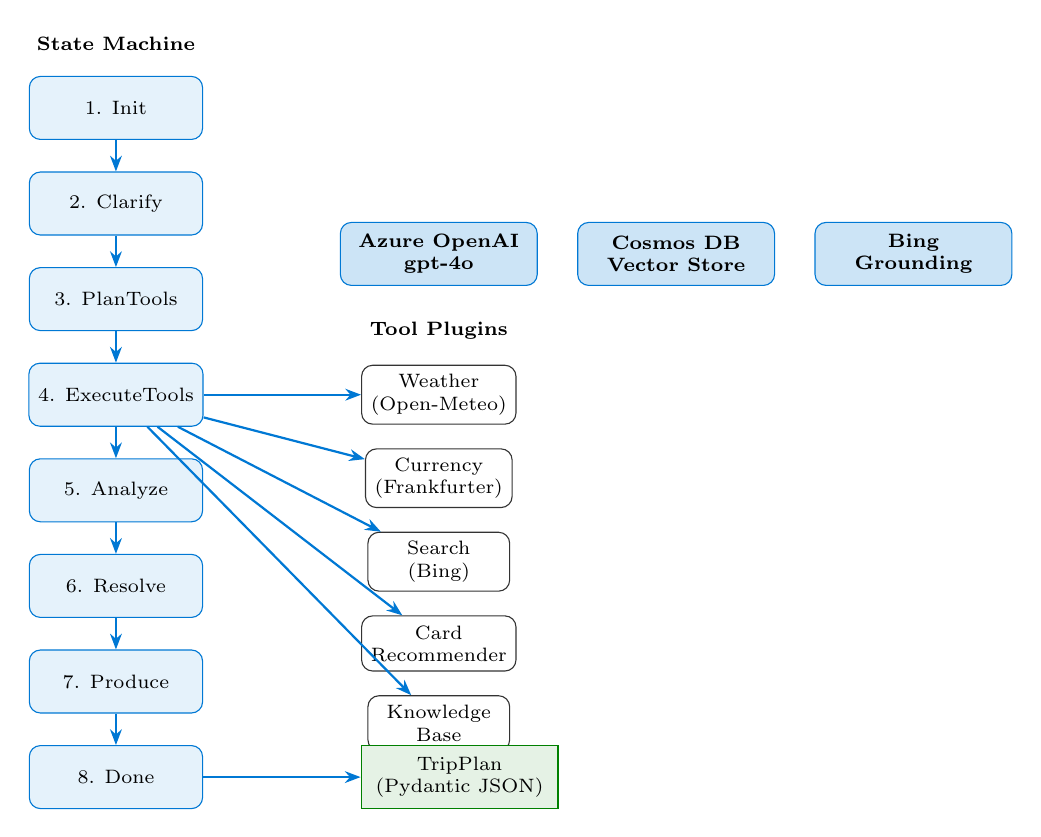
\begin{tikzpicture}[
        node distance=0.8cm and 1.5cm,
        % Styles
        phase/.style={rectangle, rounded corners, draw=azureblue, fill=azureblue!10,
                     minimum width=2.2cm, minimum height=0.8cm, align=center, font=\scriptsize},
        tool/.style={rectangle, rounded corners, draw=darkgray, fill=white,
                    minimum width=1.8cm, minimum height=0.7cm, align=center, font=\scriptsize},
        azure/.style={rectangle, rounded corners, draw=azureblue, fill=azureblue!20,
                     minimum width=2.5cm, minimum height=0.8cm, align=center, font=\scriptsize\bfseries},
        output/.style={rectangle, draw=greencolor, fill=greencolor!10,
                      minimum width=2.5cm, minimum height=0.8cm, align=center, font=\scriptsize},
        arrow/.style={-{Stealth[length=2mm]}, thick, azureblue},
    ]

    % State Machine Phases (vertical)
    \node[phase] (init) {1. Init};
    \node[phase, below=0.4cm of init] (clarify) {2. Clarify};
    \node[phase, below=0.4cm of clarify] (plan) {3. PlanTools};
    \node[phase, below=0.4cm of plan] (execute) {4. ExecuteTools};
    \node[phase, below=0.4cm of execute] (analyze) {5. Analyze};
    \node[phase, below=0.4cm of analyze] (resolve) {6. Resolve};
    \node[phase, below=0.4cm of resolve] (produce) {7. Produce};
    \node[phase, below=0.4cm of produce] (done) {8. Done};

    % Arrows between phases
    \draw[arrow] (init) -- (clarify);
    \draw[arrow] (clarify) -- (plan);
    \draw[arrow] (plan) -- (execute);
    \draw[arrow] (execute) -- (analyze);
    \draw[arrow] (analyze) -- (resolve);
    \draw[arrow] (resolve) -- (produce);
    \draw[arrow] (produce) -- (done);

    % Tools (right side)
    \node[tool, right=2cm of execute] (weather) {Weather\\(Open-Meteo)};
    \node[tool, below=0.3cm of weather] (fx) {Currency\\(Frankfurter)};
    \node[tool, below=0.3cm of fx] (search) {Search\\(Bing)};
    \node[tool, below=0.3cm of search] (card) {Card\\Recommender};
    \node[tool, below=0.3cm of card] (knowledge) {Knowledge\\Base};

    % Connect execute to tools
    \draw[arrow] (execute) -- (weather);
    \draw[arrow] (execute) -- (fx);
    \draw[arrow] (execute) -- (search);
    \draw[arrow] (execute) -- (card);
    \draw[arrow] (execute) -- (knowledge);

    % Azure Services (top right)
    \node[azure, above=1cm of weather] (aoai) {Azure OpenAI\\gpt-4o};
    \node[azure, right=0.5cm of aoai] (cosmos) {Cosmos DB\\Vector Store};
    \node[azure, right=0.5cm of cosmos] (bing) {Bing\\Grounding};

    % Output
    \node[output, right=2cm of done] (tripplan) {TripPlan\\(Pydantic JSON)};
    \draw[arrow] (done) -- (tripplan);

    % Labels
    \node[font=\scriptsize\bfseries, above=0.2cm of init] {State Machine};
    \node[font=\scriptsize\bfseries, above=0.2cm of weather] {Tool Plugins};

    \end{tikzpicture}
    \caption{AI Travel Concierge Agent Architecture}
    \label{fig:architecture}
\end{figure}

\subsection{Component Summary}

\begin{table}[H]
\centering
\caption{System Components}
\begin{tabular}{llp{7cm}}
\toprule
\textbf{Component} & \textbf{Technology} & \textbf{Purpose} \\
\midrule
Orchestration & Semantic Kernel 1.36.1 & Agent workflow and tool coordination \\
LLM & Azure OpenAI gpt-4o & Natural language understanding and generation \\
Embeddings & text-embedding-3-small & Vector embeddings for RAG retrieval \\
Vector Store & Azure Cosmos DB & Knowledge storage with vector search \\
Web Search & Bing Grounding (AI Foundry) & Real-time travel information retrieval \\
Validation & Pydantic 2.11.7 & Structured output validation (TripPlan) \\
\bottomrule
\end{tabular}
\end{table}

\newpage

% ============================================================
% AZURE RESOURCES
% ============================================================
\section{Azure Resources}

\subsection{Azure OpenAI Deployments}

The following models are deployed in the Azure AI Services resource:

\begin{figure}[H]
    \centering
    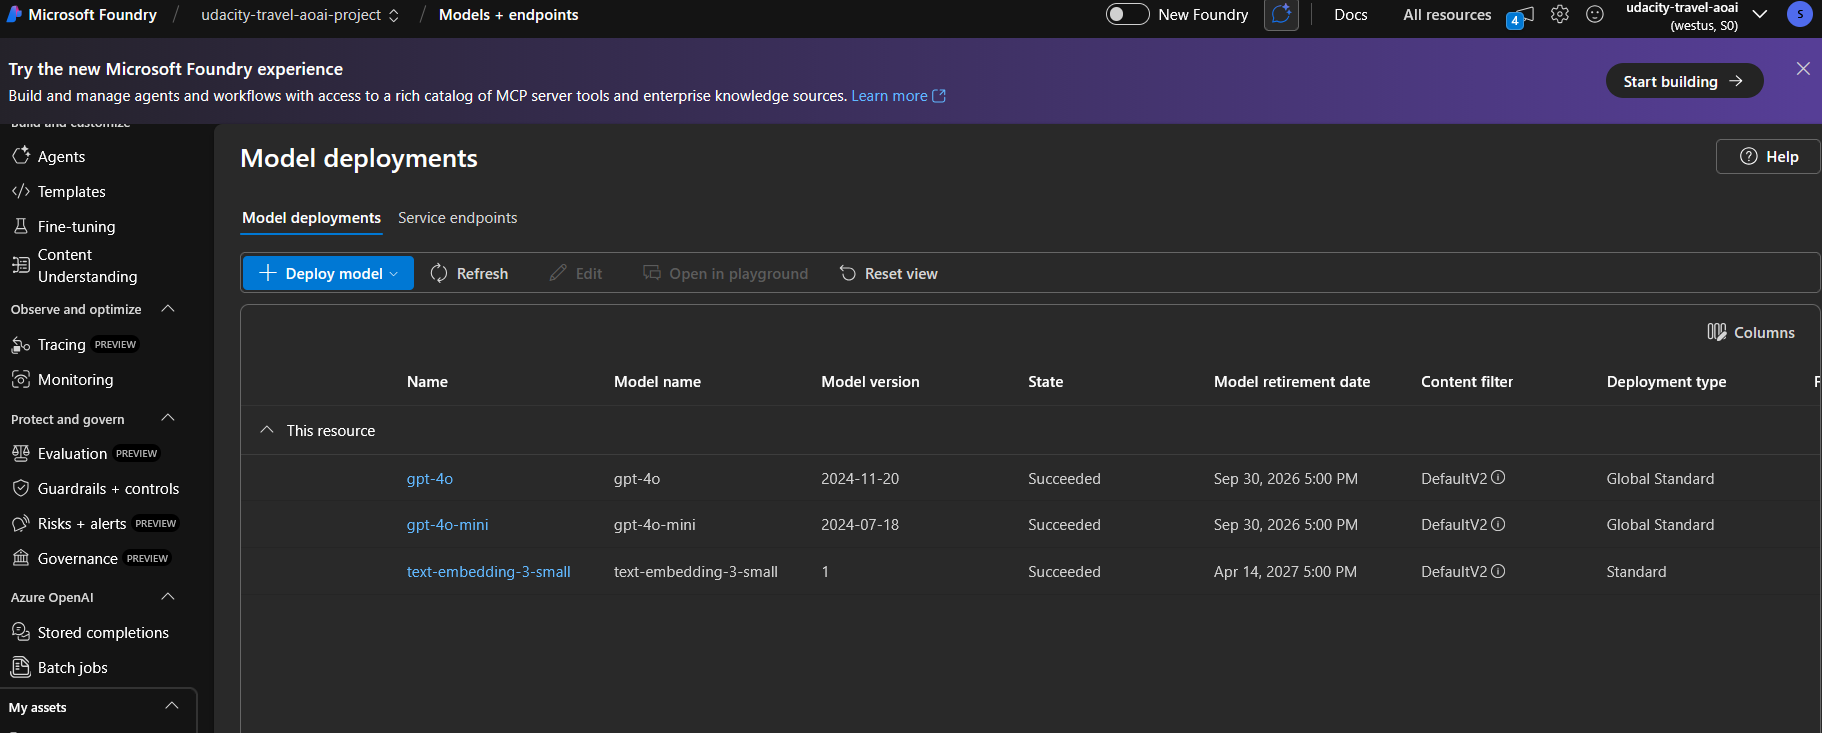
\includegraphics[width=0.95\textwidth]{Foundry_Models_Deployed.png}
    \caption{Azure OpenAI Model Deployments showing gpt-4o, gpt-4o-mini, and text-embedding-3-small}
    \label{fig:deployments}
\end{figure}

\begin{table}[H]
\centering
\caption{Model Deployment Configuration}
\begin{tabular}{llll}
\toprule
\textbf{Deployment} & \textbf{Model} & \textbf{Type} & \textbf{TPM} \\
\midrule
gpt-4o & gpt-4o & GlobalStandard & 10,000 \\
gpt-4o-mini & gpt-4o-mini & GlobalStandard & 10,000 \\
text-embedding-3-small & text-embedding-3-small & Standard & 10,000 \\
\bottomrule
\end{tabular}
\end{table}

\subsection{Azure Cosmos DB}

Vector-enabled Cosmos DB stores knowledge snippets with embeddings for RAG retrieval:

\begin{figure}[H]
    \centering
    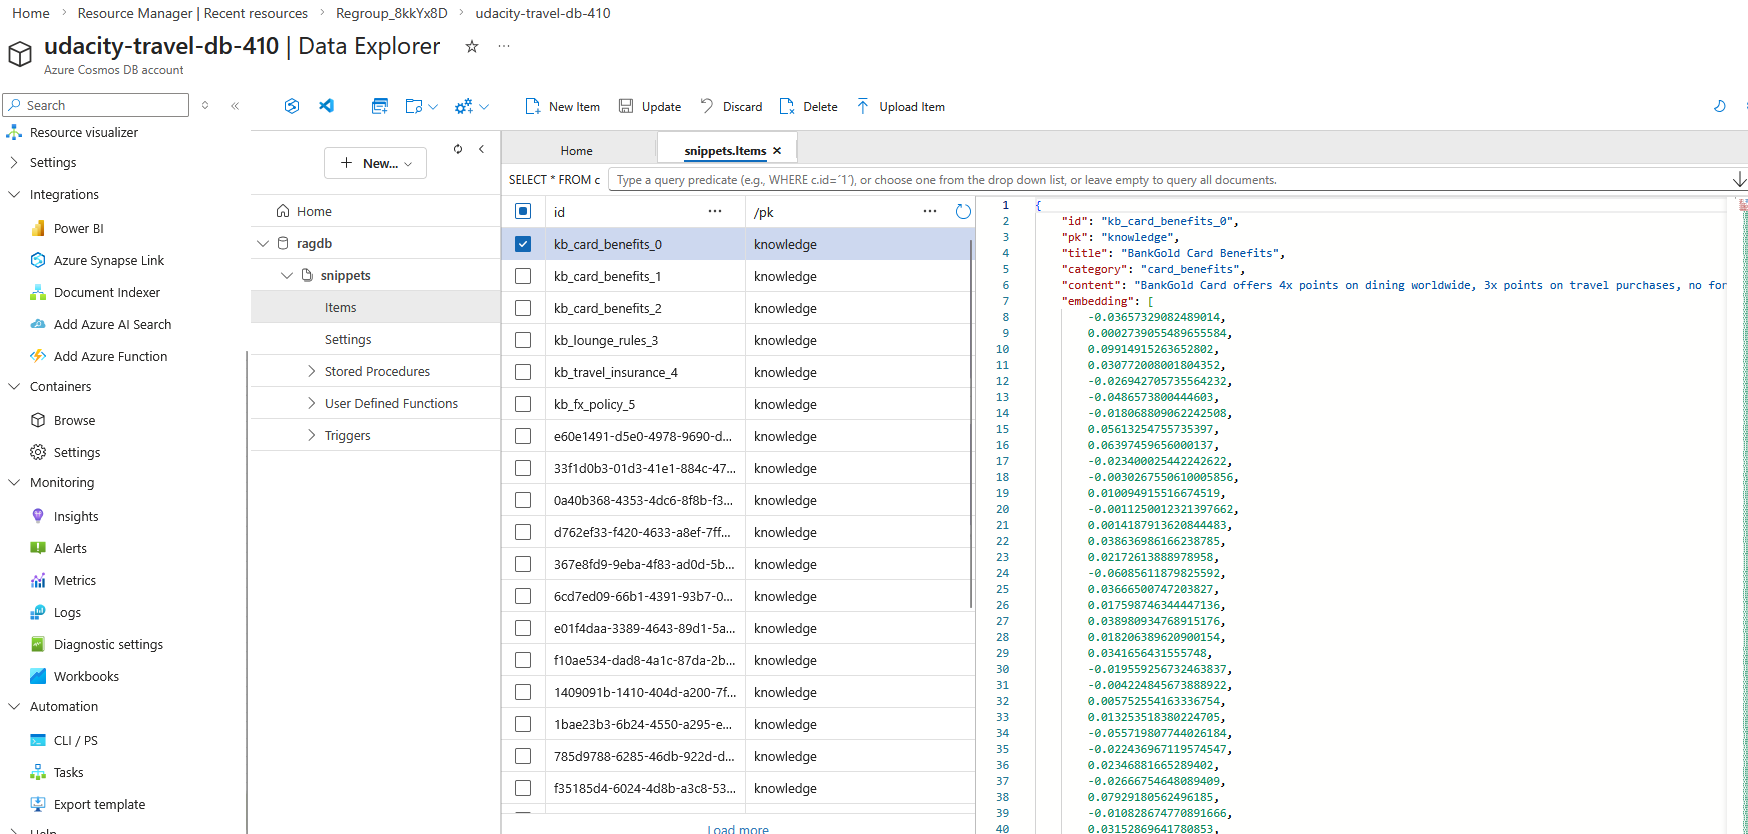
\includegraphics[width=0.95\textwidth]{Cosmos_db_items.png}
    \caption{Cosmos DB Data Explorer showing knowledge snippets with embedding vectors}
    \label{fig:cosmos}
\end{figure}

\begin{table}[H]
\centering
\caption{Cosmos DB Configuration}
\begin{tabular}{ll}
\toprule
\textbf{Setting} & \textbf{Value} \\
\midrule
Account Name & udacity-travel-db-410 \\
Database & ragdb \\
Container & snippets \\
Partition Key & /pk \\
Capacity Mode & Serverless \\
Region & West US \\
\bottomrule
\end{tabular}
\end{table}

\newpage

\subsection{Azure AI Foundry Agent with Bing Grounding}

The Travel Concierge Agent uses Azure AI Foundry with Bing Grounding for real-time web search:

\begin{figure}[H]
    \centering
    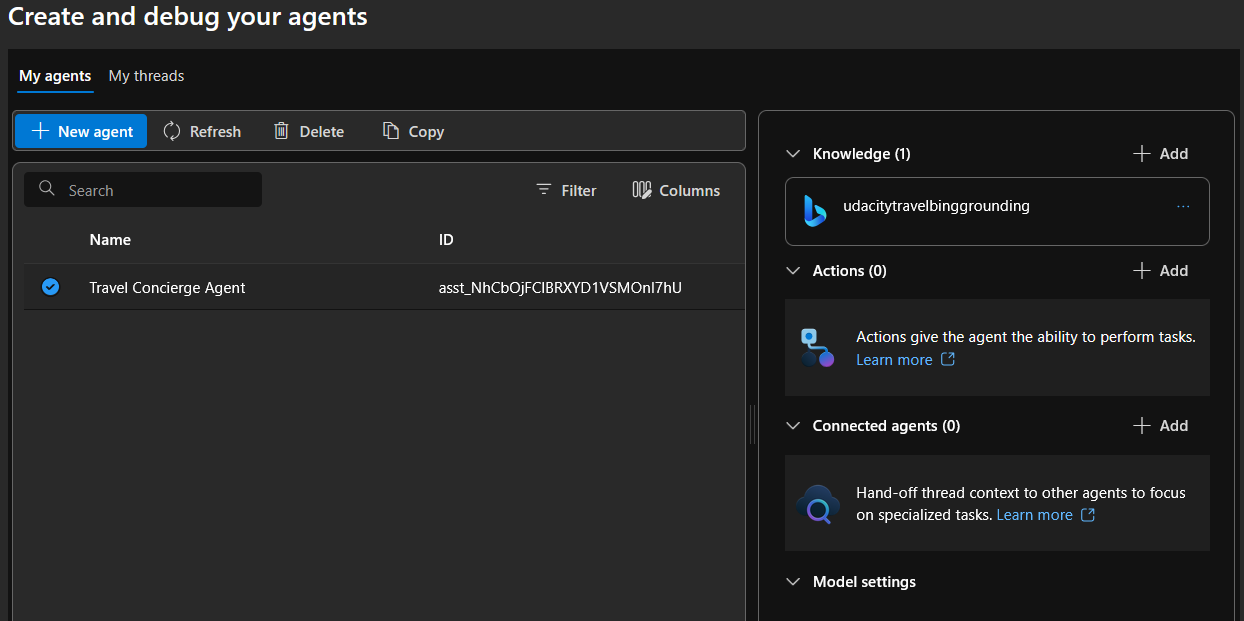
\includegraphics[width=0.95\textwidth]{Foundry_Agent_Bing.png}
    \caption{Azure AI Foundry Agent with Bing Search tool connected}
    \label{fig:bing}
\end{figure}

\begin{table}[H]
\centering
\caption{AI Foundry Agent Configuration}
\begin{tabular}{ll}
\toprule
\textbf{Setting} & \textbf{Value} \\
\midrule
Project Name & udacity-travel-aoai-project \\
Agent Name & Travel Concierge Agent \\
Agent ID & asst\_NhCbOjFClBRXYD1VSMOnI7hU \\
Model & gpt-4o \\
Tool & Bing Grounding (Search) \\
\bottomrule
\end{tabular}
\end{table}

\begin{figure}[H]
    \centering
    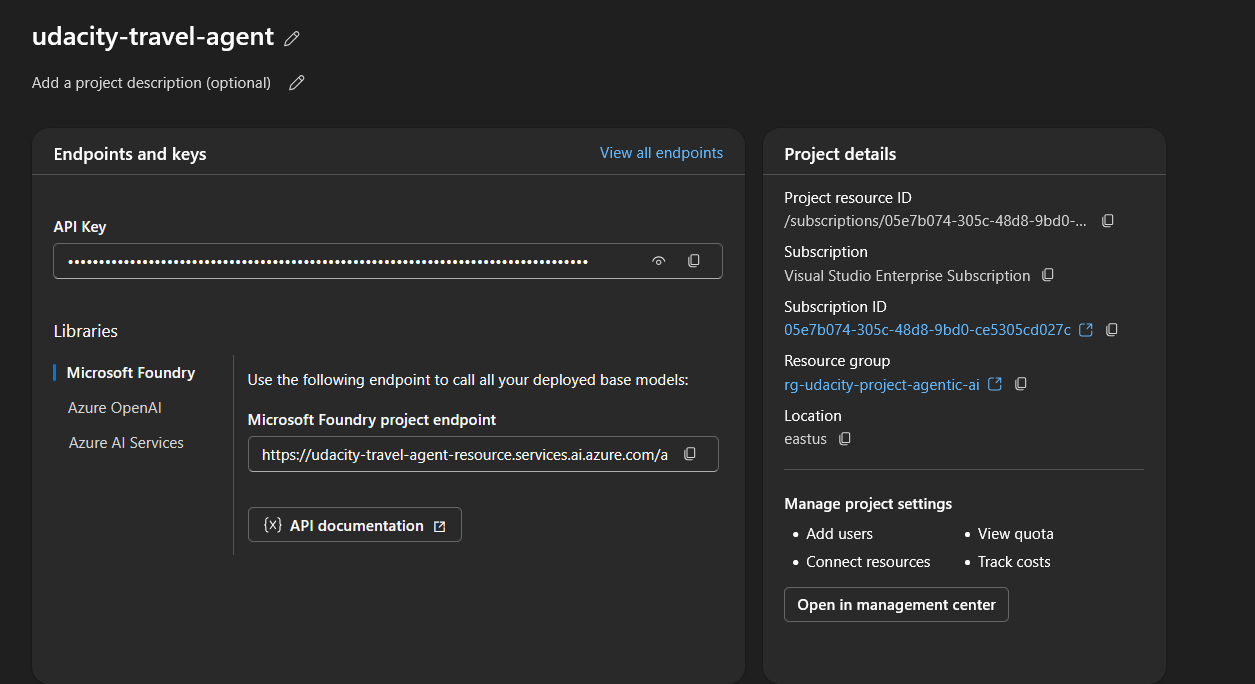
\includegraphics[width=0.95\textwidth]{Foundry_Project_Overview.png}
    \caption{Azure AI Foundry Project Overview}
    \label{fig:foundry}
\end{figure}

\newpage

% ============================================================
% TEST RESULTS
% ============================================================
\section{Test Results}

\subsection{Unit Tests}

All 76 unit tests pass successfully:

\begin{table}[H]
\centering
\caption{Unit Test Results by Module}
\begin{tabular}{lcc}
\toprule
\textbf{Test Module} & \textbf{Tests} & \textbf{Status} \\
\midrule
test\_models.py & 12 & PASS \\
test\_state.py & 24 & PASS \\
test\_memory.py & 18 & PASS \\
test\_memory\_integration.py & 14 & PASS \\
test\_tools.py & 8 & PASS \\
\midrule
\textbf{Total} & \textbf{76} & \textbf{All Passing} \\
\bottomrule
\end{tabular}
\end{table}

\subsection{System Health Check}

The system check validates all components are properly configured:

\begin{figure}[H]
    \centering
    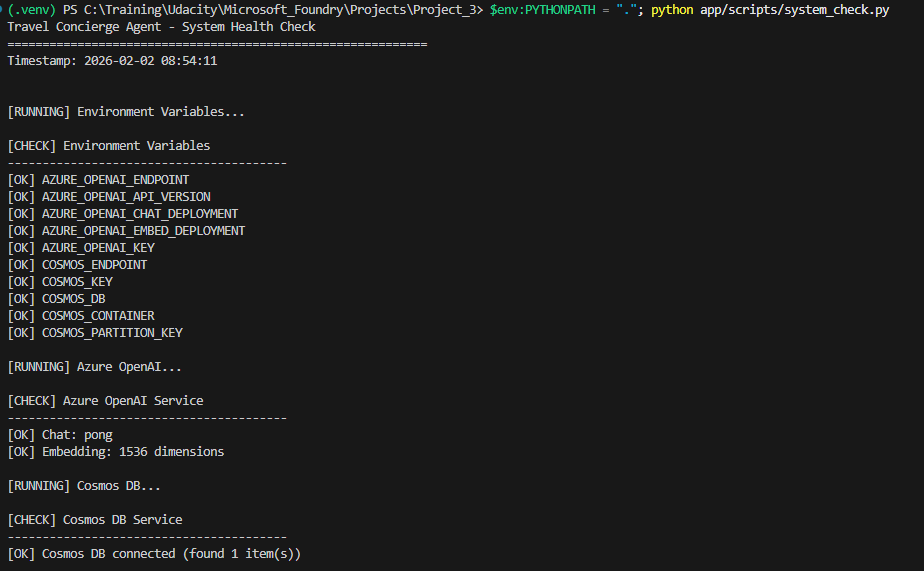
\includegraphics[width=0.95\textwidth]{System_checks_passed_1.png}
    \caption{System Health Check Results (Part 1)}
    \label{fig:syscheck1}
\end{figure}

\begin{figure}[H]
    \centering
    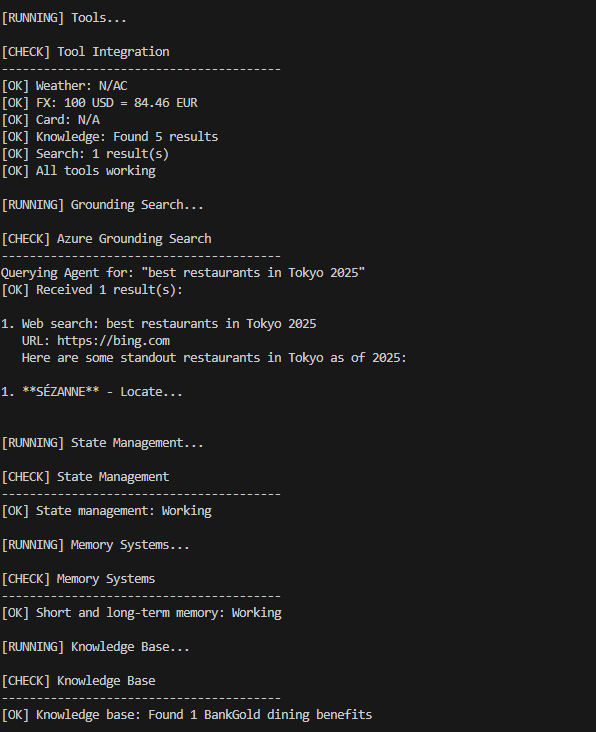
\includegraphics[width=0.95\textwidth]{System_checks_passed_2.png}
    \caption{System Health Check Results (Part 2)}
    \label{fig:syscheck2}
\end{figure}

\begin{figure}[H]
    \centering
    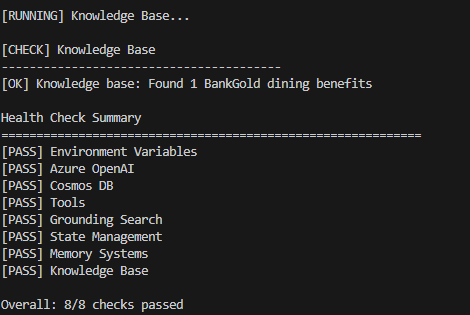
\includegraphics[width=0.95\textwidth]{System_checks_passed_3.png}
    \caption{System Health Check Results (Part 3)}
    \label{fig:syscheck3}
\end{figure}

\begin{table}[H]
\centering
\caption{System Check Results Summary}
\begin{tabular}{lc}
\toprule
\textbf{Check} & \textbf{Status} \\
\midrule
Environment Variables & PASS \\
Azure OpenAI Connection & PASS \\
Cosmos DB Connection & PASS \\
Tools (Weather, FX, Search, Card, Knowledge) & PASS \\
Grounding Search (Bing via AI Foundry) & PASS \\
State Management (8-phase workflow) & PASS \\
Memory Systems (Short-term + Long-term) & PASS \\
Knowledge Base (Card benefits retrieval) & PASS \\
\midrule
\textbf{Total} & \textbf{8/8 Passed} \\
\bottomrule
\end{tabular}
\end{table}

\newpage

% ============================================================
% LLM JUDGE EVALUATION
% ============================================================
\section{LLM-as-Judge Evaluation}

The agent was evaluated using an LLM-as-Judge approach with weighted scoring across six criteria:

\begin{figure}[H]
    \centering
    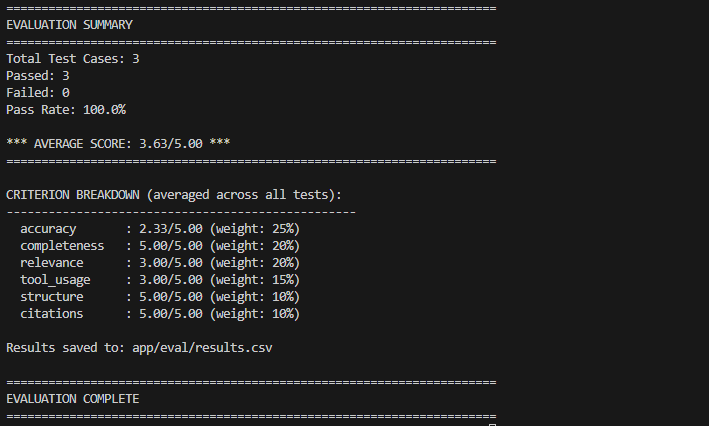
\includegraphics[width=0.95\textwidth]{LLM_Evaluation_Overview.png}
    \caption{LLM-as-Judge Evaluation Output}
    \label{fig:llmjudge}
\end{figure}

\subsection{Evaluation Criteria and Weights}

\begin{table}[H]
\centering
\caption{LLM Judge Scoring Criteria}
\begin{tabular}{lcp{7cm}}
\toprule
\textbf{Criterion} & \textbf{Weight} & \textbf{Description} \\
\midrule
Accuracy & 25\% & Factual correctness of information provided \\
Completeness & 20\% & All required fields populated in TripPlan \\
Relevance & 20\% & Response addresses user's specific query \\
Tool Usage & 15\% & Appropriate tools called for the request \\
Structure & 10\% & Valid JSON conforming to Pydantic schema \\
Citations & 10\% & Sources provided for factual claims \\
\bottomrule
\end{tabular}
\end{table}

\subsection{Evaluation Results}

Three test cases were evaluated:

\begin{enumerate}
    \item Paris trip (June 2026) with BankGold card
    \item Tokyo trip (March 2026) with BankPremium card
    \item Barcelona trip (August 2026) with BankRewards card
\end{enumerate}

\begin{table}[H]
\centering
\caption{LLM Judge Scores by Criterion}
\begin{tabular}{lcc}
\toprule
\textbf{Criterion} & \textbf{Average Score} & \textbf{Weight} \\
\midrule
Accuracy & 2.33/5.00 & 25\% \\
Completeness & 5.00/5.00 & 20\% \\
Relevance & 3.00/5.00 & 20\% \\
Tool Usage & 3.00/5.00 & 15\% \\
Structure & 5.00/5.00 & 10\% \\
Citations & 5.00/5.00 & 10\% \\
\midrule
\textbf{Overall} & \textbf{3.63/5.00} & 100\% \\
\bottomrule
\end{tabular}
\end{table}

\begin{table}[H]
\centering
\caption{Evaluation Summary}
\begin{tabular}{ll}
\toprule
\textbf{Metric} & \textbf{Value} \\
\midrule
Total Test Cases & 3 \\
Passed & 3 \\
Failed & 0 \\
Pass Rate & 100\% \\
Average Score & 3.63/5.00 \\
\bottomrule
\end{tabular}
\end{table}

\newpage

% ============================================================
% RAG IMPLEMENTATION
% ============================================================
\section{RAG Implementation}

\subsection{Knowledge Base}

The RAG system stores travel-related knowledge in Cosmos DB with vector embeddings:

\begin{figure}[H]
    \centering
    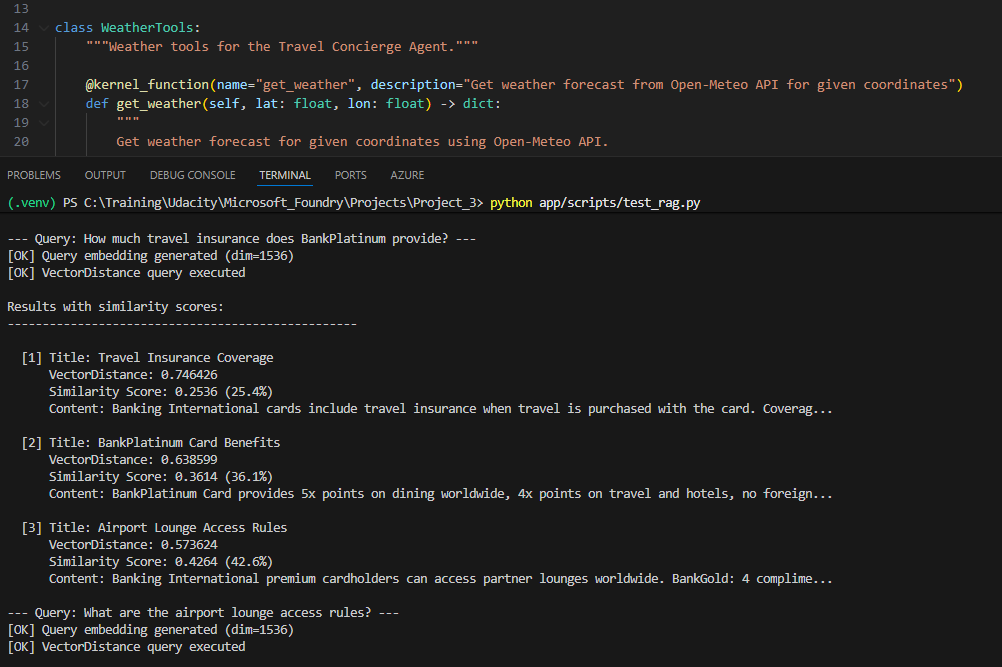
\includegraphics[width=0.95\textwidth]{RAG_Scores_Examples.png}
    \caption{RAG Retrieval with Vector Similarity Scores}
    \label{fig:rag}
\end{figure}

\begin{table}[H]
\centering
\caption{Knowledge Base Content}
\begin{tabular}{lp{8cm}}
\toprule
\textbf{Category} & \textbf{Content} \\
\midrule
Card Benefits & BankGold: 4x dining, 3x travel, no FX fees \\
Card Benefits & BankPremium: 5x dining, 4x travel, lounge access \\
Card Benefits & BankRewards: 3x on all purchases, 1.5\% cashback \\
Lounge Rules & Priority Pass access requirements \\
Travel Policies & Insurance coverage details \\
MCC Benefits & Category-specific reward multipliers \\
\bottomrule
\end{tabular}
\end{table}

\subsection{Embedding Configuration}

\begin{lstlisting}[language=Python]
# Embedding generation using Azure OpenAI
embedding_service = AzureTextEmbedding(
    deployment_name="text-embedding-3-small",
    endpoint=os.getenv("AZURE_OPENAI_ENDPOINT"),
    api_key=os.getenv("AZURE_OPENAI_API_KEY"),
    api_version="2024-02-15-preview"
)

# Generate embeddings for knowledge snippets
embeddings = await embedding_service.generate_embeddings([text])
\end{lstlisting}

\subsection{RAG Ingestion Results}

\begin{lstlisting}[basicstyle=\ttfamily\small]
[START] Starting knowledge base ingestion...
[OK] Embedding service initialized
[OK] Connected to Cosmos DB: ragdb/snippets
[OK] Upserted snippet: bankgold-benefits
[OK] Upserted snippet: bankpremium-benefits
[OK] Upserted snippet: bankrewards-benefits
[OK] Upserted snippet: lounge-rules
[OK] Upserted snippet: travel-insurance
[OK] Upserted snippet: dining-mcc
[OK] Upserted snippet: hotel-mcc
[OK] Ingested 7 documents
\end{lstlisting}

\newpage

% ============================================================
% CODE IMPLEMENTATION
% ============================================================
\section{Key Implementation Details}

\subsection{8-Phase State Machine}

The agent follows a structured workflow through 8 phases:

\begin{lstlisting}[language=Python]
class AgentPhase(Enum):
    """Agent workflow phases"""
    Init = "Init"
    ClarifyRequirements = "ClarifyRequirements"
    PlanTools = "PlanTools"
    ExecuteTools = "ExecuteTools"
    AnalyzeResults = "AnalyzeResults"
    ResolveIssues = "ResolveIssues"
    ProduceStructuredOutput = "ProduceStructuredOutput"
    Done = "Done"
\end{lstlisting}

\subsection{Tool Integration}

Five tools are registered as Semantic Kernel plugins:

\begin{lstlisting}[language=Python]
# Register tool plugins
kernel.add_plugin(WeatherTools(), plugin_name="WeatherTools")
kernel.add_plugin(FxTools(), plugin_name="FxTools")
kernel.add_plugin(SearchTools(), plugin_name="SearchTools")
kernel.add_plugin(CardTools(), plugin_name="CardTools")
kernel.add_plugin(KnowledgeTools(), plugin_name="KnowledgeTools")
\end{lstlisting}

\subsection{Pydantic Output Validation}

The TripPlan output is validated using Pydantic:

\begin{lstlisting}[language=Python]
class TripPlan(BaseModel):
    """Validated trip plan output"""
    destination: str
    dates: TravelDates
    weather: WeatherInfo
    currency: CurrencyInfo
    recommendations: List[Recommendation]
    card_recommendation: CardRecommendation
    citations: List[Citation]
\end{lstlisting}

\subsection{Bing Grounding Integration}

Web search uses Azure AI Foundry Agent with Bing tool:

\begin{lstlisting}[language=Python]
# Create AI Foundry Agent client
project_client = AIProjectClient(
    credential=DefaultAzureCredential(),
    endpoint=os.getenv("PROJECT_ENDPOINT")
)

# Execute search via agent
thread = project_client.agents.create_thread_and_process_run(
    assistant_id=os.getenv("AGENT_ID"),
    thread={"messages": [{"role": "user", "content": query}]}
)
\end{lstlisting}

\newpage

% ============================================================
% CONCLUSIONS
% ============================================================
\section{Conclusions}

This project successfully implements an AI Travel Concierge Agent using Semantic Kernel with Azure AI services. Key achievements include:

\begin{enumerate}
    \item \textbf{Agentic Architecture}: 8-phase state machine with proper workflow management
    \item \textbf{Tool Integration}: Five tools (Weather, Currency, Search, Card, Knowledge) as SK plugins
    \item \textbf{RAG Implementation}: Vector embeddings stored in Cosmos DB with similarity search
    \item \textbf{Bing Grounding}: Real-time web search via Azure AI Foundry Agent
    \item \textbf{Structured Output}: Pydantic-validated TripPlan JSON schema
    \item \textbf{LLM Evaluation}: 3.63/5.00 average score with 100\% pass rate
    \item \textbf{Comprehensive Testing}: 76 unit tests + 8/8 system checks passing
\end{enumerate}

\subsection{Technology Stack Summary}

\begin{table}[H]
\centering
\begin{tabular}{ll}
\toprule
\textbf{Component} & \textbf{Implementation} \\
\midrule
Orchestration & Semantic Kernel 1.36.1 \\
LLM & Azure OpenAI gpt-4o, gpt-4o-mini \\
Embeddings & text-embedding-3-small (1536 dimensions) \\
Vector Store & Azure Cosmos DB (serverless) \\
Web Search & Bing Grounding via AI Foundry Agent \\
Weather API & Open-Meteo (free, no auth) \\
Currency API & Frankfurter (free, no auth) \\
Validation & Pydantic 2.11.7 \\
Testing & pytest with 76 tests \\
\bottomrule
\end{tabular}
\end{table}

\subsection{Repository}

All code is available at: \url{https://github.com/rodolfolermacontreras/-Udacity-Foundry-Project3}

\vspace{1cm}

\begin{center}
\textit{End of Submission Report}
\end{center}

\end{document}
